\section{The \emph{Compact Muon Solenoid} experiment}
%%%%%%%%%%%%%%%%%%%%%%%%%%%%%%%%%%%%%%%%%
\label{sec:CMS}

The CMS apparatus is a general purpose detector situated in one of the four LHC interaction points\footnote{The CMS detector is placed in a cavern 100\,m underground in the area called Point 5, near the village of Cessy, in France.}. The detector is designed to investigate a wide range of physics, from the search of the Higgs boson, to SM measurements and BSM physics searches. To achieve this goal, the detector is able to identify and reconstruct all the physics objects that may be produced in the proton proton collisions: electrons, muons, photons and jets. The main feature of the CMS detector is a superconducting solenoidal magnet which is capable to produce a $3.8$\,T magnetic field. Such a strong magnetic field is the key aspect which permits to have a compact design of the detector. The detector has a cylindrical structure, which is typical of general purpose detectors, which consists of several cylindrical detecting layers, coaxial with the beam direction (\emph{barrel} region), closed at both ends with detecting disks (\emph{endcap} region), in such a way to ensure the hermetic closure of the apparatus.

The coordinate system used by CMS is a right-handed Cartesian system, with the origin in the nominal beam collision point inside the detector. The $x$-axis is chose to point radially towards the center of the LHC circumference and the $y$-axis is directed upwards along the vertical. The $z$-axis is oriented along the beam direction, according to the counter-clockwise direction of the LHC ring if seen from above. The CMS cylindrical symmetry and the Lorentz invariant description of the proton proton collisions, suggest the use of a pseudo-angular reference frame, described by the triplet of coordinates $(r,\phi,\eta)$, where $r$ is the distance from the $z$-axis, $\phi$ is the azimuthal angle, measured starting from the $x$-axis positive direction, and $\eta$ is the pseudorapidity, defined by the following equation:
\begin{equation}
\eta = - \ln\left( \tan\frac{\theta}{2}\right) \quad,
\end{equation}
where $\theta$ is the polar angle. The used of pseudorapidity is preferred over the polar angle because differences in pseudorapidity are Lorentz invariant under boosts along the $z$-axis. In the limit of ultrarelativistic particles the pseudorapidity coincides with the rapidity $y$:
\begin{equation}
y = \frac{1}{2}\ln\left(\frac{E+p_z}{E-p_z}\right) \quad ,
\end{equation}
where $E$ is the particle energy and $p_z$ is the momentum projection along the $z$-axis.

The schematic view of the CMS detector, which has a length of 21.5\,m, a diameter of 15\,m and a weight of about $14000$\,tons, is shown in Fig.~\ref{fig:CMS}. From the inner region to the outer one, the various CMS sub-detectors are:
\begin{itemize}
\item {\bf Silicon tracker}: it occupies the region $r < 1.2$\,m and $|\eta|<2.5$. It is composed of an inner silicon pixel vertex detector and a surrounding silicon microstrip detector, with a total active area of about $215\,\mathrm{m^2}$. It is used to reconstruct charged particle tracks and vertices;
\item {\bf Electromagnetic calorimeter (ECAL)}: placed in the region $1.2\,\mathrm{m} < r < 1.8\,\mathrm{m}$ and $|\eta|<3$, it consists of many scintillating crystals of lead tungstate ($\mathrm{PbWO_4}$). It is used for the measurement of the trajectory and the energy released by electrons and photons;
\item {\bf Hadronic calorimeter (HCAL)}: it is placed in the region $1.8\,\mathrm{m} < r < 2.9\,\mathrm{m}$ and $|\eta|<5$. It is made up of brass layers alternated with plastic scintillators and it is used to measure the direction and energy deposited by the hadrons produced in the interactions;
\item {\bf Superconducting solenoidal magnet}: it occupies the region $2.9\,\mathrm{m} < r < 3.8\,\mathrm{m}$ and $|\eta|<1.5$ and generates an internal uniform magnetic field with an intensity of 3.8\,T, pointing along the direction of the beams. The magnetic field is necessary to bend the trajectories of charged particles, in order to allow the measurement of their momentum through the curvature observed in the tracking system. The magnetic field lines are closed by an external 21\,m long iron yoke, that has a diameter of 14\,m. Outside the return yoke, a residual 1.8\,T magnetic field is present, pointing in the opposite direction with respect to the internal field;
\item {\bf Muon system}: the outermost system, which is placed in the region $4\,\mathrm{m} < r < 7.4\,\mathrm{m}$ and $|\eta|<2.4$, has the purpose of reconstructing the tracks of muons passing through it. It consists of Drift Tubes (DT) in the barrel region and Cathode Strip Chambers (CSC) in the endcaps. A complementary system of Resistive Plate Chambers (RPC) is used both in the barrel and endcaps. The muon chambers are housed inside the iron structure of the return yoke.
\end{itemize}

\begin{figure}[htb]
\centering
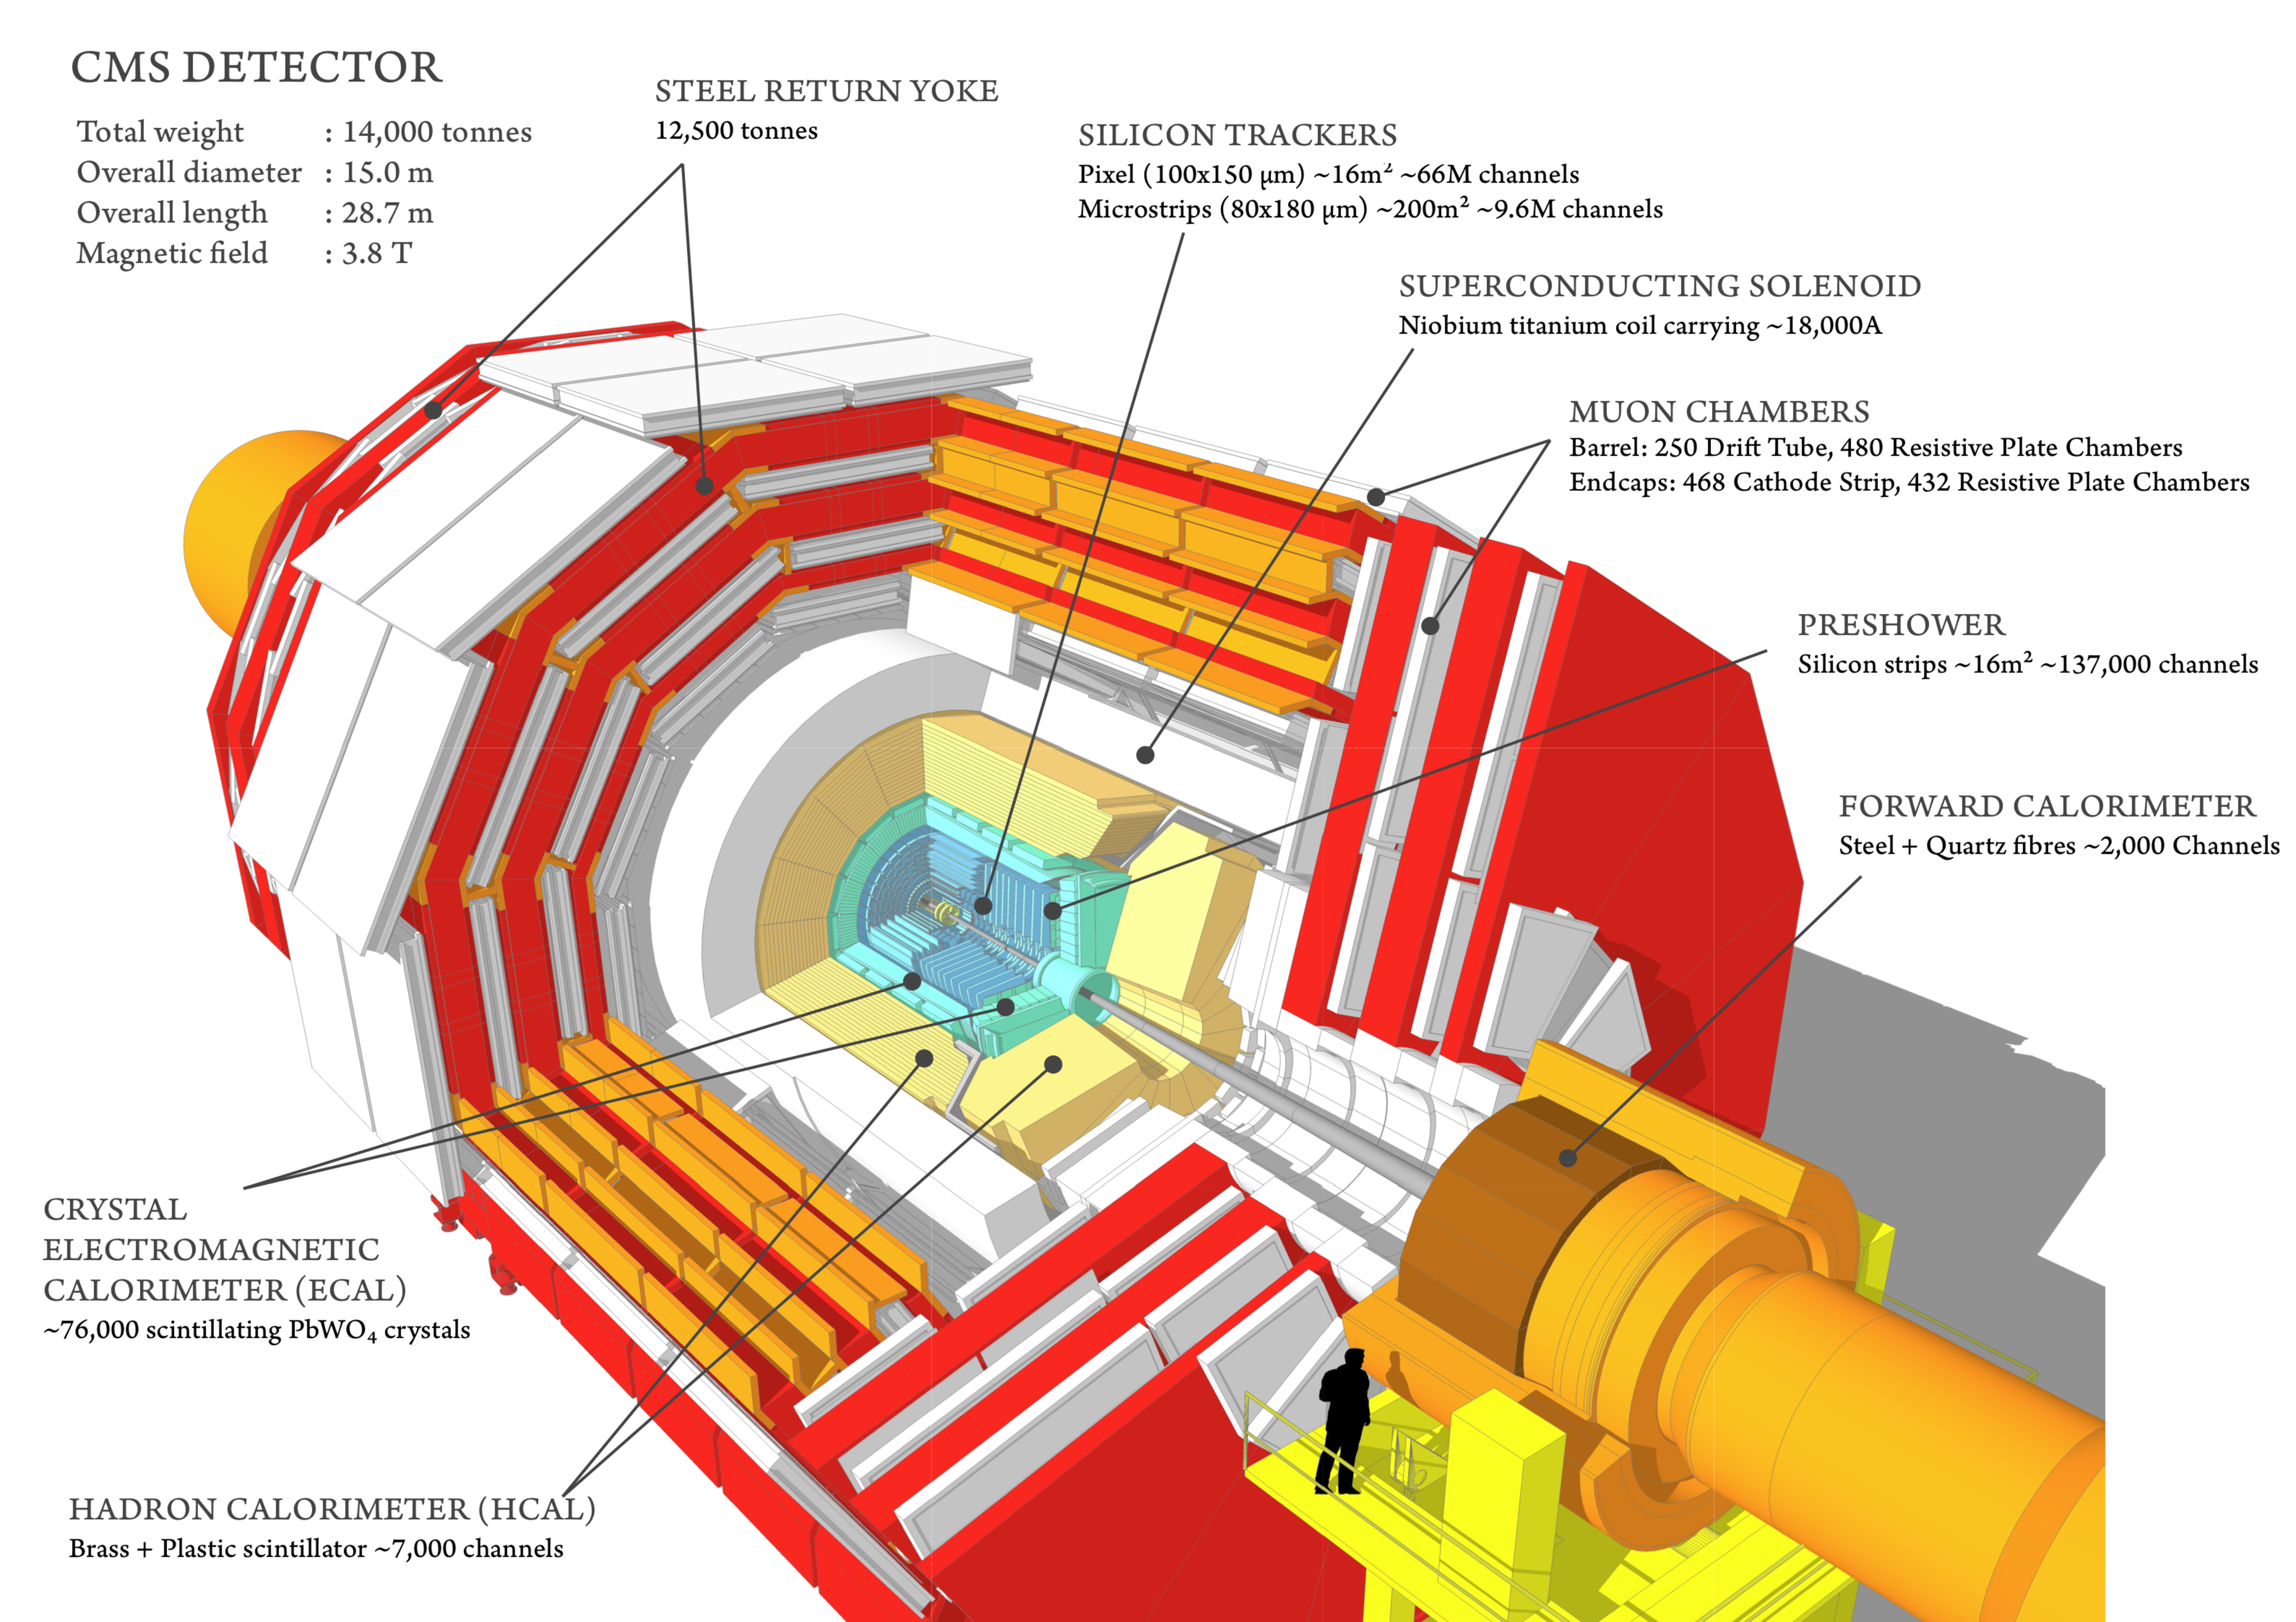
\includegraphics[width=0.7\textwidth]{images/CMS.pdf}
\caption{Schematic view of the CMS detector showing its sub-detectors.}\label{fig:CMS}
\end{figure}
\begin{figure}[htb]
\centering
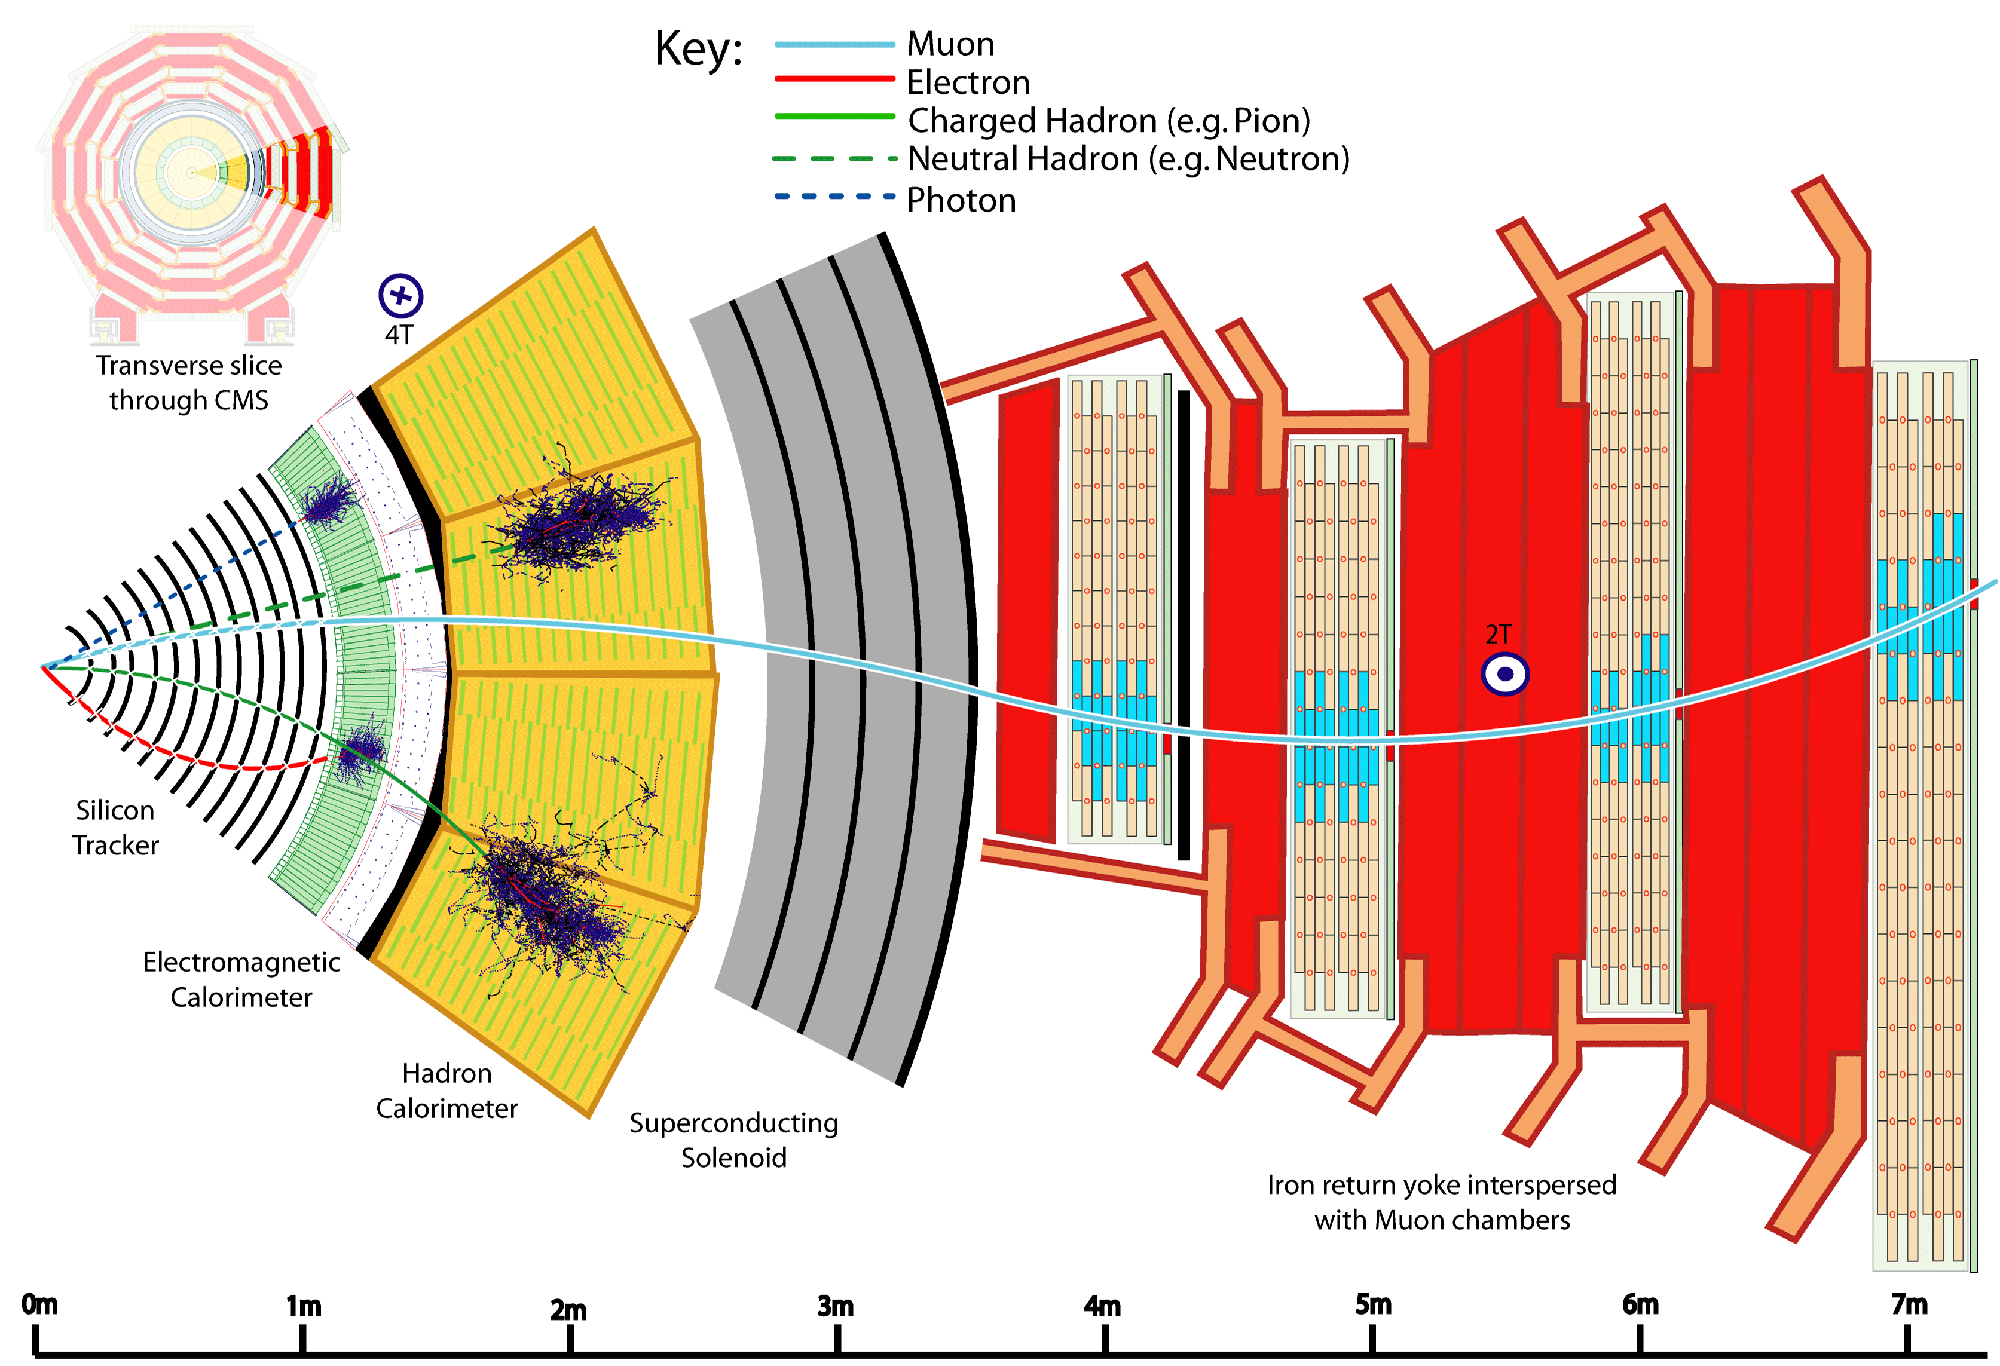
\includegraphics[width=0.7\textwidth]{images/CMSslice.png}
\caption{Schematic view of a slice of the CMS detector, showing the sub-detectors response to the passage of different types of particles.}\label{fig:CMSslice}
\end{figure}

In Fig.~\ref{fig:CMSslice} the response of the various CMS sub-detectors to the passage of different types of particles is sketched. In the following sections a brief description of each sub-detector is given.

\subsection{The tracker}

	\subsubsection{The pixel detector}

	\subsubsection{The microstrip detector}


\subsection{The electromagnetic calorimeter (ECAL)}

\subsection{The hadronic calorimeter (HCAL)}

\subsection{The solenoid}

\subsection{The muon system}

